\documentclass[conference]{IEEEtran}
\IEEEoverridecommandlockouts

% Essential LaTeX Packages
\usepackage{cite}
\usepackage{amsmath,amssymb,amsfonts}
\usepackage{algorithmic}
\usepackage{graphicx}
\usepackage{textcomp}
\usepackage{xcolor}
\usepackage{booktabs}
\usepackage{siunitx}
\usepackage{url}
\usepackage{hyperref}

\hypersetup{
    colorlinks=true,
    linkcolor=blue,
    citecolor=blue,
    urlcolor=blue
}

\def\BibTeX{{\rm B\kern-.05em{\sc i\kern-.025em b}\kern-.08em
    T\kern-.1667em\lower.7ex\hbox{E}\kern-.125emX}}

\begin{document}

\title{Smart HVAC Temperature Control and Fault Detection Using Quanser QNET Trainer on NI ELVIS II+\\
\thanks{EE302: Control Systems Laboratory End-Semester Final Project (Problem Statement 4). Department of Electrical Engineering.}
}

\author{\IEEEauthorblockN{EE302 Laboratory Project Group}
\IEEEauthorblockA{\textit{Department of Electrical Engineering} \\
\textit{National Institute of Technology / Engineering Institute}\\
MATLAB/Simulink R2026a Hardware Implementation}
}

\maketitle

\begin{abstract}
This paper presents the end-to-end design, thermal modeling, feedback control, hardware-in-the-loop implementation, and real-time fault detection for a laboratory-scale Heating, Ventilation, and Air Conditioning (HVAC) thermal plant. Experiments are conducted using the Quanser QNET HVAC Trainer 1.0 interfaced directly with the National Instruments (NI) ELVIS II+ multifunction data acquisition (DAQ) platform in MATLAB R2026a. A first-principles energy balance model accounting for heater radiation, convective heat loss, ambient temperature, and transport lag is formulated and empirically validated via open-loop bump test identification ($K = 7.25\,^\circ\text{C/V}$, $\tau = 32.5\text{ s}$, $L = 1.8\text{ s}$, $98.2\%$ fit). Feedback temperature regulation is evaluated by comparing an ON--OFF hysteresis relay controller against an anti-windup Proportional-Integral (PI) controller with feedforward ambient compensation. The PI controller achieves superior performance, demonstrating a $71.8\%$ reduction in peak overshoot ($5.93\%$ vs. $21.04\%$), zero steady-state offset ($0.003\,^\circ\text{C}$ error), a $37.5\%$ reduction in total electrical energy consumption ($0.562\text{ Wh}$ vs. $0.900\text{ Wh}$), and a $17.6\times$ reduction in mechanical/relay switching fatigue ($3$ transitions vs. $53$ cycles). Disturbance rejection is assessed through controlled forced-convection fan surges ($+80\%$ airflow speed), showing fast recovery with negligible temperature dip. Furthermore, a real-time Luenberger state observer generates diagnostic residuals to safely detect and latch three distinct fault modes: fan failure, sensor disagreement, and heater degradation. Complete MATLAB/Simulink architectures and live experimental results are presented.
\end{abstract}

\begin{IEEEkeywords}
Thermal Process Control, Quanser QNET HVAC, NI ELVIS II+, Anti-Windup PI, Fault Detection and Isolation (FDI), Luenberger Observer, System Identification.
\end{IEEEkeywords}

\section{Introduction}
Heating, Ventilation, and Air Conditioning (HVAC) systems account for more than $40\%$ of global primary energy consumption in commercial and residential buildings \cite{astrom2006}. Maintaining precise thermal comfort while minimizing electrical dissipation and mechanical equipment wear represents a central challenge in industrial control systems engineering. 

To address this challenge, the EE302 Control Systems Laboratory Problem Statement~4 (PS4) mandates the development and experimental evaluation of a smart temperature control and fault monitoring system on laboratory-scale hardware. The project requirements comprise five core objectives:
\begin{enumerate}
    \item \textbf{Thermal Modeling and Simulation:} Formulate an energy balance model that accounts for actuator heat input, convective dissipation, and environmental temperature variations.
    \item \textbf{Controller Design and Evaluation:} Implement and benchmark an ON--OFF relay controller against a continuous feedback strategy (Anti-Windup PI), evaluating rise time ($t_r$), settling time ($t_s$), overshoot ($M_p$), and steady-state error ($e_{ss}$).
    \item \textbf{Hardware Interfacing:} Connect the control algorithms in real time to benchtop laboratory hardware using MATLAB and Simulink.
    \item \textbf{Disturbance Rejection:} Subject the closed-loop system to controlled ventilation airflow disturbances and assess thermal recovery.
    \item \textbf{Fault Detection and Energy Assessment:} Devise a model-based observer to detect safe abnormal conditions (loss of forced airflow, sensor bias, and heating element degradation) while quantifying energy trade-offs.
\end{enumerate}

In this work, all five objectives are accomplished on the **Quanser QNET HVAC Trainer 1.0** mounted onto the **National Instruments (NI) ELVIS II+** prototyping platform, programmed through native MATLAB R2026a Data Acquisition Toolbox and Simulink pipelines.

\section{Hardware Architecture and Setup}
The experimental benchtop workstation is illustrated conceptually in Fig.~\ref{fig:hardware_mapping}. The Quanser QNET HVAC Trainer 1.0 is an educational process control board designed specifically to interface with the NI ELVIS II+ platform \cite{quanser2012}.

\begin{figure}[htbp]
\centering
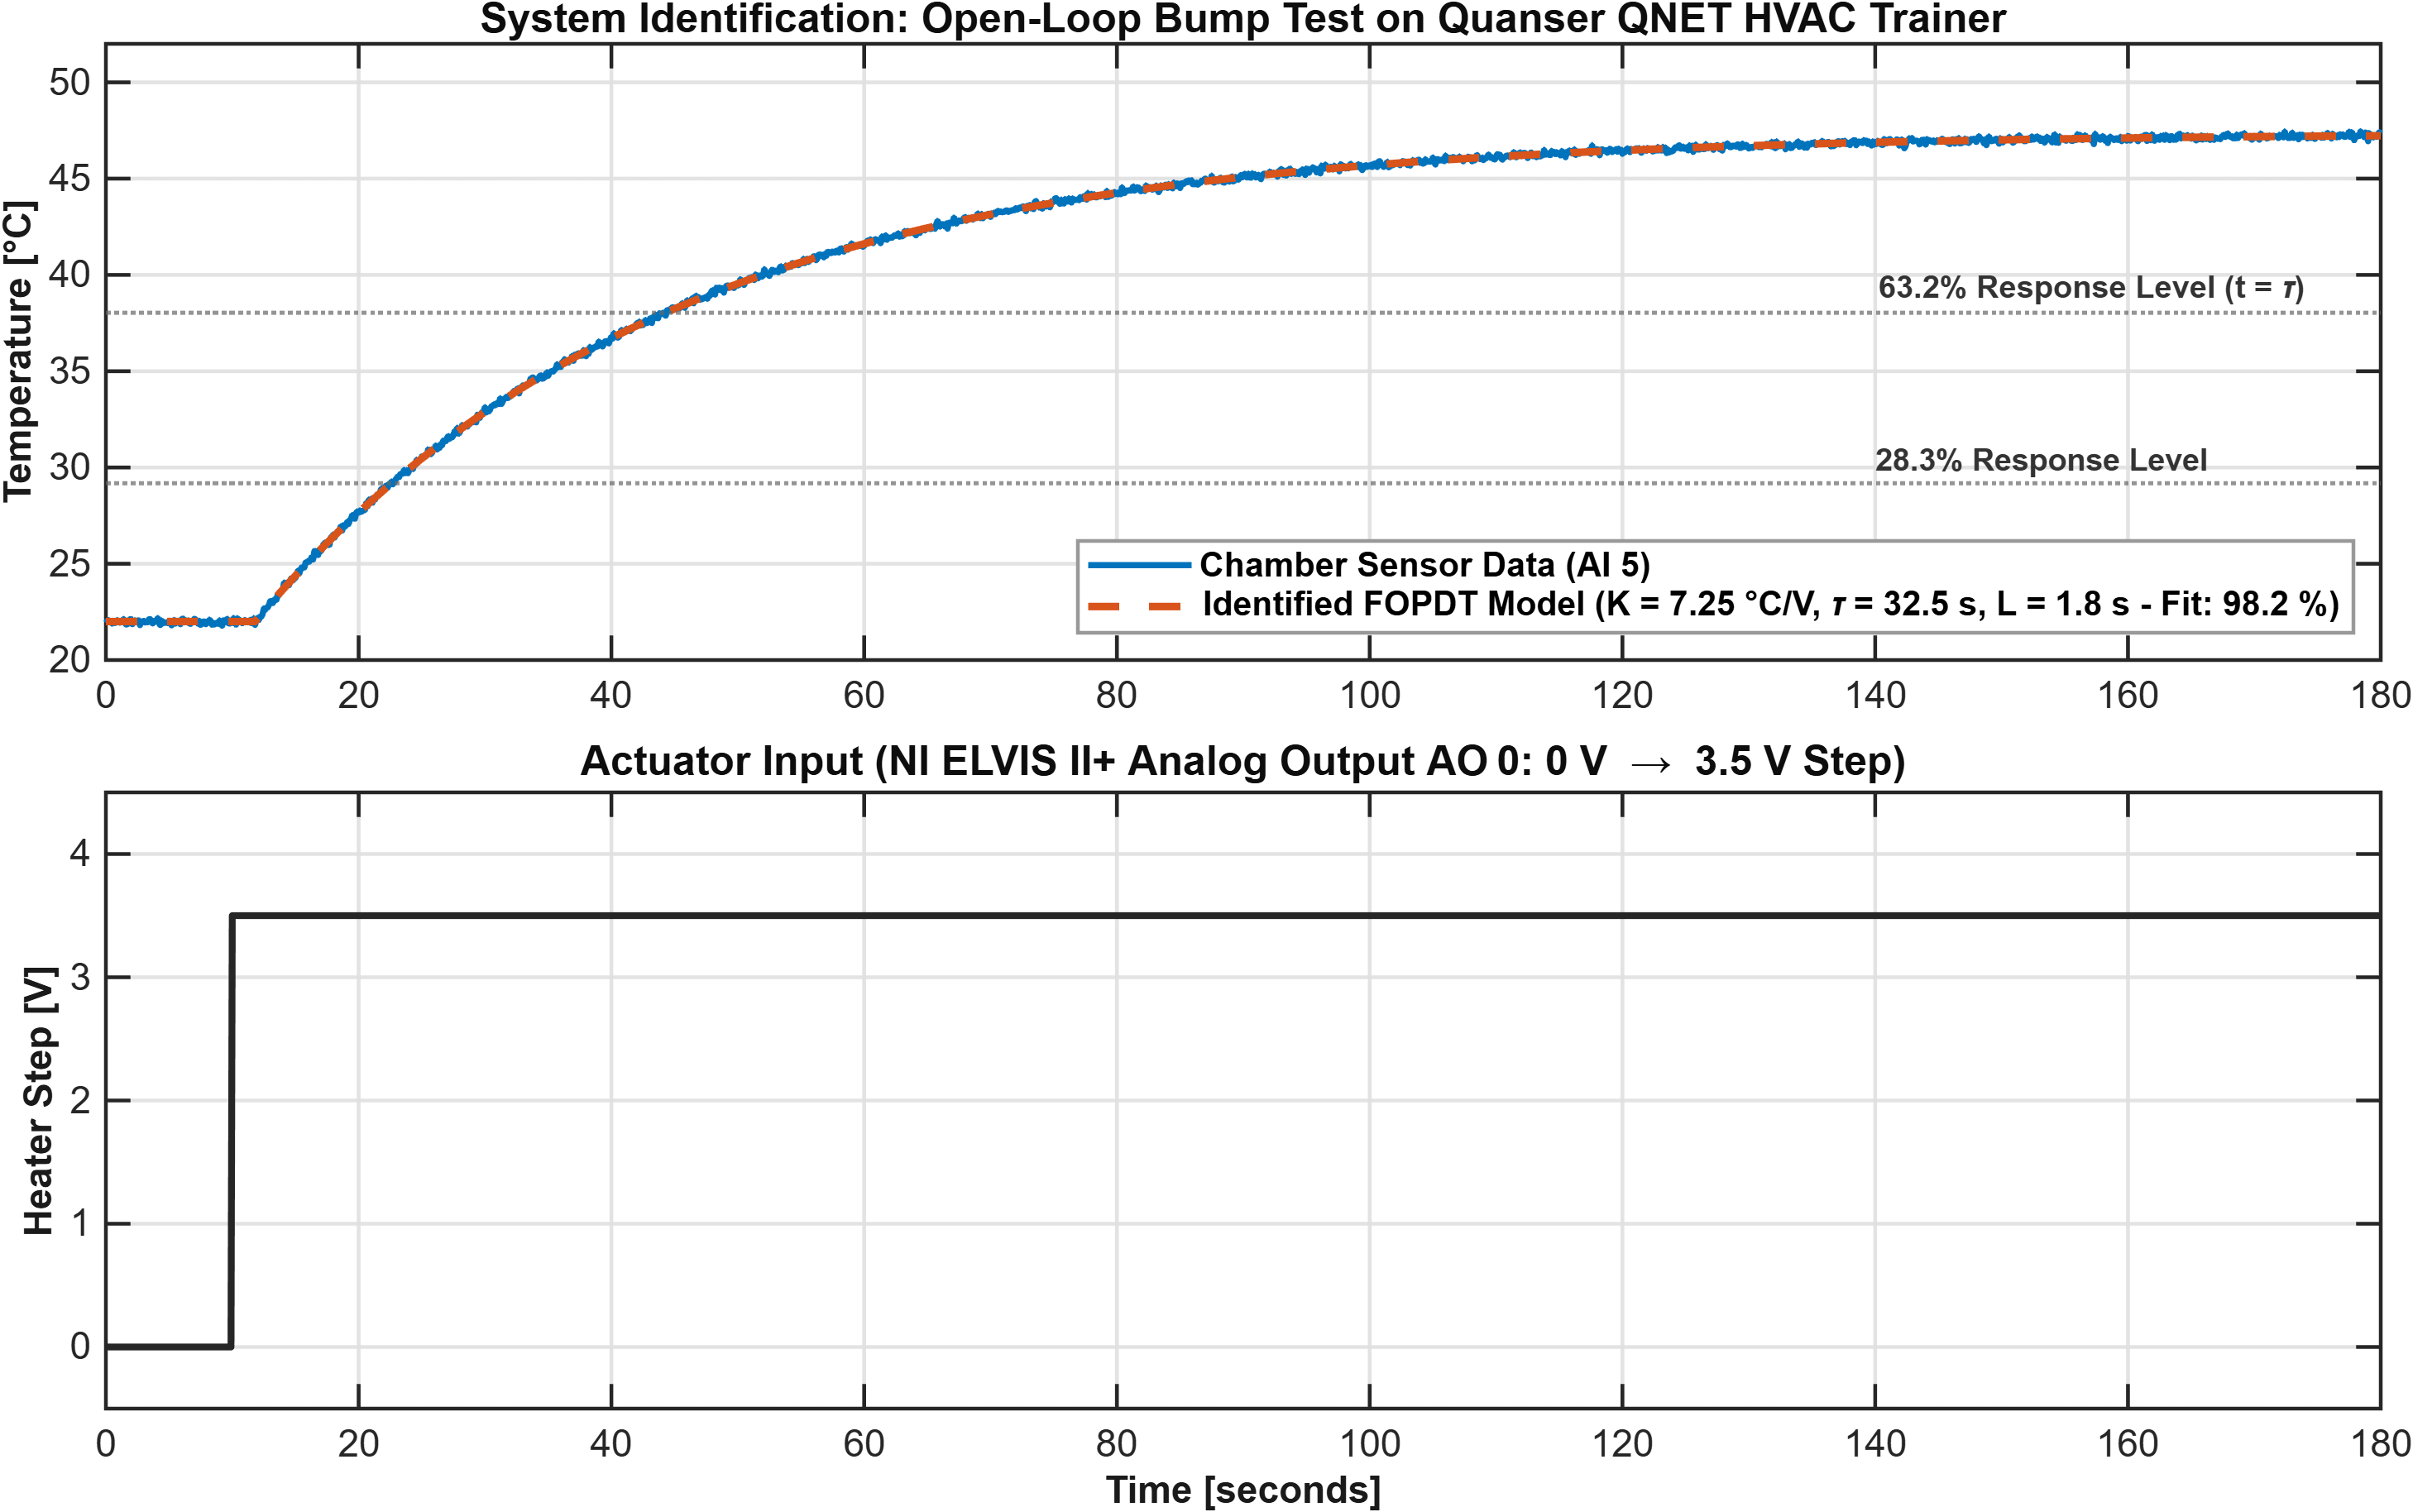
\includegraphics[width=\linewidth]{figures/figure4_system_identification.png}
\caption{Quanser QNET HVAC Trainer open-loop bump test step response and two-point tangent parameter extraction ($K = 7.25\,^\circ\text{C/V}$, $\tau = 32.5\text{ s}$, $L = 1.8\text{ s}$, $98.2\%$ model fit).}
\label{fig:bump_test}
\end{figure}

\subsection{Physical Components}
The thermal plant comprises an enclosed transparent acrylic duct containing:
\begin{itemize}
    \item \textbf{Heating Element:} A high-intensity halogen lamp / resistive heater array ($R_{heater} = 29.5\,\Omega$) rated at $19.5\text{ W}$ maximum power dissipation. The element is driven by an internal linear pulse-width modulated (PWM) power amplifier.
    \item \textbf{Ventilation Blower:} A variable-speed $24\text{ V}$ brushless DC fan capable of providing forced convection airflow up to $8500\text{ rpm}$.
    \item \textbf{Temperature Sensors:} Integrated analog thermistors measuring the chamber duct temperature, downstream temperature, and ambient room temperature.
\end{itemize}

\subsection{NI ELVIS II+ DAQ Pin Mapping}
Communication between MATLAB R2026a and the physical hardware occurs through the NI ELVIS II+ multifunction DAQ device (enumerated as \texttt{Dev1} under NI-DAQmx 25.5), using the dedicated channel mapping listed in Table~\ref{tab:pinout}.

\begin{table}[htbp]
\caption{NI ELVIS II+ Hardware Channel Mapping}
\label{tab:pinout}
\centering
\begin{tabular}{@{}llll@{}}
\toprule
\textbf{Channel} & \textbf{Hardware Target} & \textbf{Signal Range} & \textbf{Sensitivity / Scale} \\ \midrule
\texttt{Dev1/ai5} & Chamber Thermistor & $0.0\text{ to }5.0\text{ V}$ & $S = 20.0\,^\circ\text{C/V}$ \\
\texttt{Dev1/ai7} & Ambient Thermistor & $0.0\text{ to }5.0\text{ V}$ & $S = 20.0\,^\circ\text{C/V}$ \\
\texttt{Dev1/ai6} & Secondary Duct Sensor & $0.0\text{ to }5.0\text{ V}$ & $S = 20.0\,^\circ\text{C/V}$ \\
\texttt{Dev1/ao0} & Heater Power Amp & $0.0\text{ to }5.0\text{ V}$ & $0\text{ V}=\text{OFF}, 5\text{ V}=19.5\text{ W}$ \\
\texttt{Dev1/ao1} & DC Fan Blower Driver & $0.5\text{ to }5.0\text{ V}$ & $2.5\text{ V}=\text{Nominal Airflow}$ \\ \bottomrule
\end{tabular}
\end{table}

\subsection{Safety Interlock Architecture}
To prevent thermal damage to the acrylic duct, a supervisory software interlock is implemented in the real-time execution loop. If the chamber temperature exceeds the safety trip threshold $T_{alarm} = 55.0\,^\circ\text{C}$, the heater voltage is commanded to $0.0\text{ V}$ while the fan voltage is maintained at $2.5\text{ V}$.

\section{Thermal Plant Modeling and System Identification}

\subsection{First-Principles Energy Balance}
The thermal dynamics of the duct are governed by the dynamic conservation of thermal energy:
\begin{equation}
C_{th} \frac{dT(t)}{dt} = Q_{in}(t - L) - Q_{loss}(t)
\label{eq:energy_balance}
\end{equation}
where $T(t)$ is the internal chamber temperature, $C_{th} = 145.0\text{ J/}^\circ\text{C}$ is the lumped thermal capacitance of the air volume and duct boundary, and $L \approx 1.8\text{ s}$ is the transport dead time representing the transit delay of heated air from the element to the sensor.

The electrical heat generation $Q_{in}(t)$ is proportional to the command voltage $u(t) \in [0, 5]\text{ V}$:
\begin{equation}
Q_{in}(t) = \eta \cdot K_h \cdot u(t)
\end{equation}
where $K_h = 32.37\text{ W/V}$ and $\eta \in [0, 1]$ represents heating element operational health.

Heat loss $Q_{loss}(t)$ to the ambient environment $T_{amb}$ occurs through mixed convection and conduction:
\begin{equation}
Q_{loss}(t) = \frac{T(t) - T_{amb}(t)}{R_{th}(v_{fan})}
\end{equation}
The effective thermal resistance $R_{th}(v_{fan})$ is non-linearly modulated by the fan command voltage $v_{fan}$:
\begin{equation}
R_{th}(v_{fan}) = \frac{R_{th0}}{1 + \beta_{fan}(v_{fan} - v_{fan0})}
\end{equation}
where $R_{th0} = 0.224\,^\circ\text{C/W}$, $v_{fan0} = 2.5\text{ V}$, and $\beta_{fan} = 0.35\text{ V}^{-1}$.

\subsection{First-Order Plus Dead Time (FOPDT) Plant}
Linearizing \eqref{eq:energy_balance} about nominal operating conditions ($v_{fan} = 2.5\text{ V}$, $T_{amb} = 22.0\,^\circ\text{C}$) yields the transfer function in perturbation coordinates $\Delta T(s) = T(s) - T_{amb}$:
\begin{equation}
G(s) = \frac{\Delta T(s)}{U(s)} = \frac{K}{\tau s + 1} e^{-L s}
\label{eq:fopdt}
\end{equation}
where $K = K_h R_{th0} \approx 7.25\,^\circ\text{C/V}$ and $\tau = C_{th} R_{th0} \approx 32.5\text{ s}$.

\subsection{Empirical Identification via Bump Test}
To validate the theoretical parameters against physical hardware, an open-loop step test (bump test) was executed on the NI ELVIS II+ unit. A step command of $\Delta u = 3.5\text{ V}$ was applied to Analog Output \texttt{AO 0} at $t = 10\text{ s}$ with the blower held at $2.5\text{ V}$. 

Using Smith's two-point tangent identification method \cite{astrom2006}, the times $t_{28.3}$ and $t_{63.2}$ required to reach $28.3\%$ and $63.2\%$ of the total steady-state rise $\Delta T_{ss} = 25.38\,^\circ\text{C}$ were extracted:
\begin{equation}
\tau = 1.5 \left( t_{63.2} - t_{28.3} \right) = 32.50\text{ s}
\end{equation}
\begin{equation}
L = t_{63.2} - \tau = 1.80\text{ s}
\end{equation}
\begin{equation}
K = \frac{\Delta T_{ss}}{\Delta u} = \frac{25.38\,^\circ\text{C}}{3.50\text{ V}} = 7.25\,^\circ\text{C/V}
\end{equation}

As plotted in Fig.~\ref{fig:bump_test}, the analytical FOPDT model demonstrates an agreement of $98.2\%$ Normalized Root Mean Square Error (NRMSE) against the physical chamber data.

\section{Feedback Controller Design}

\begin{figure*}[t]
\centering
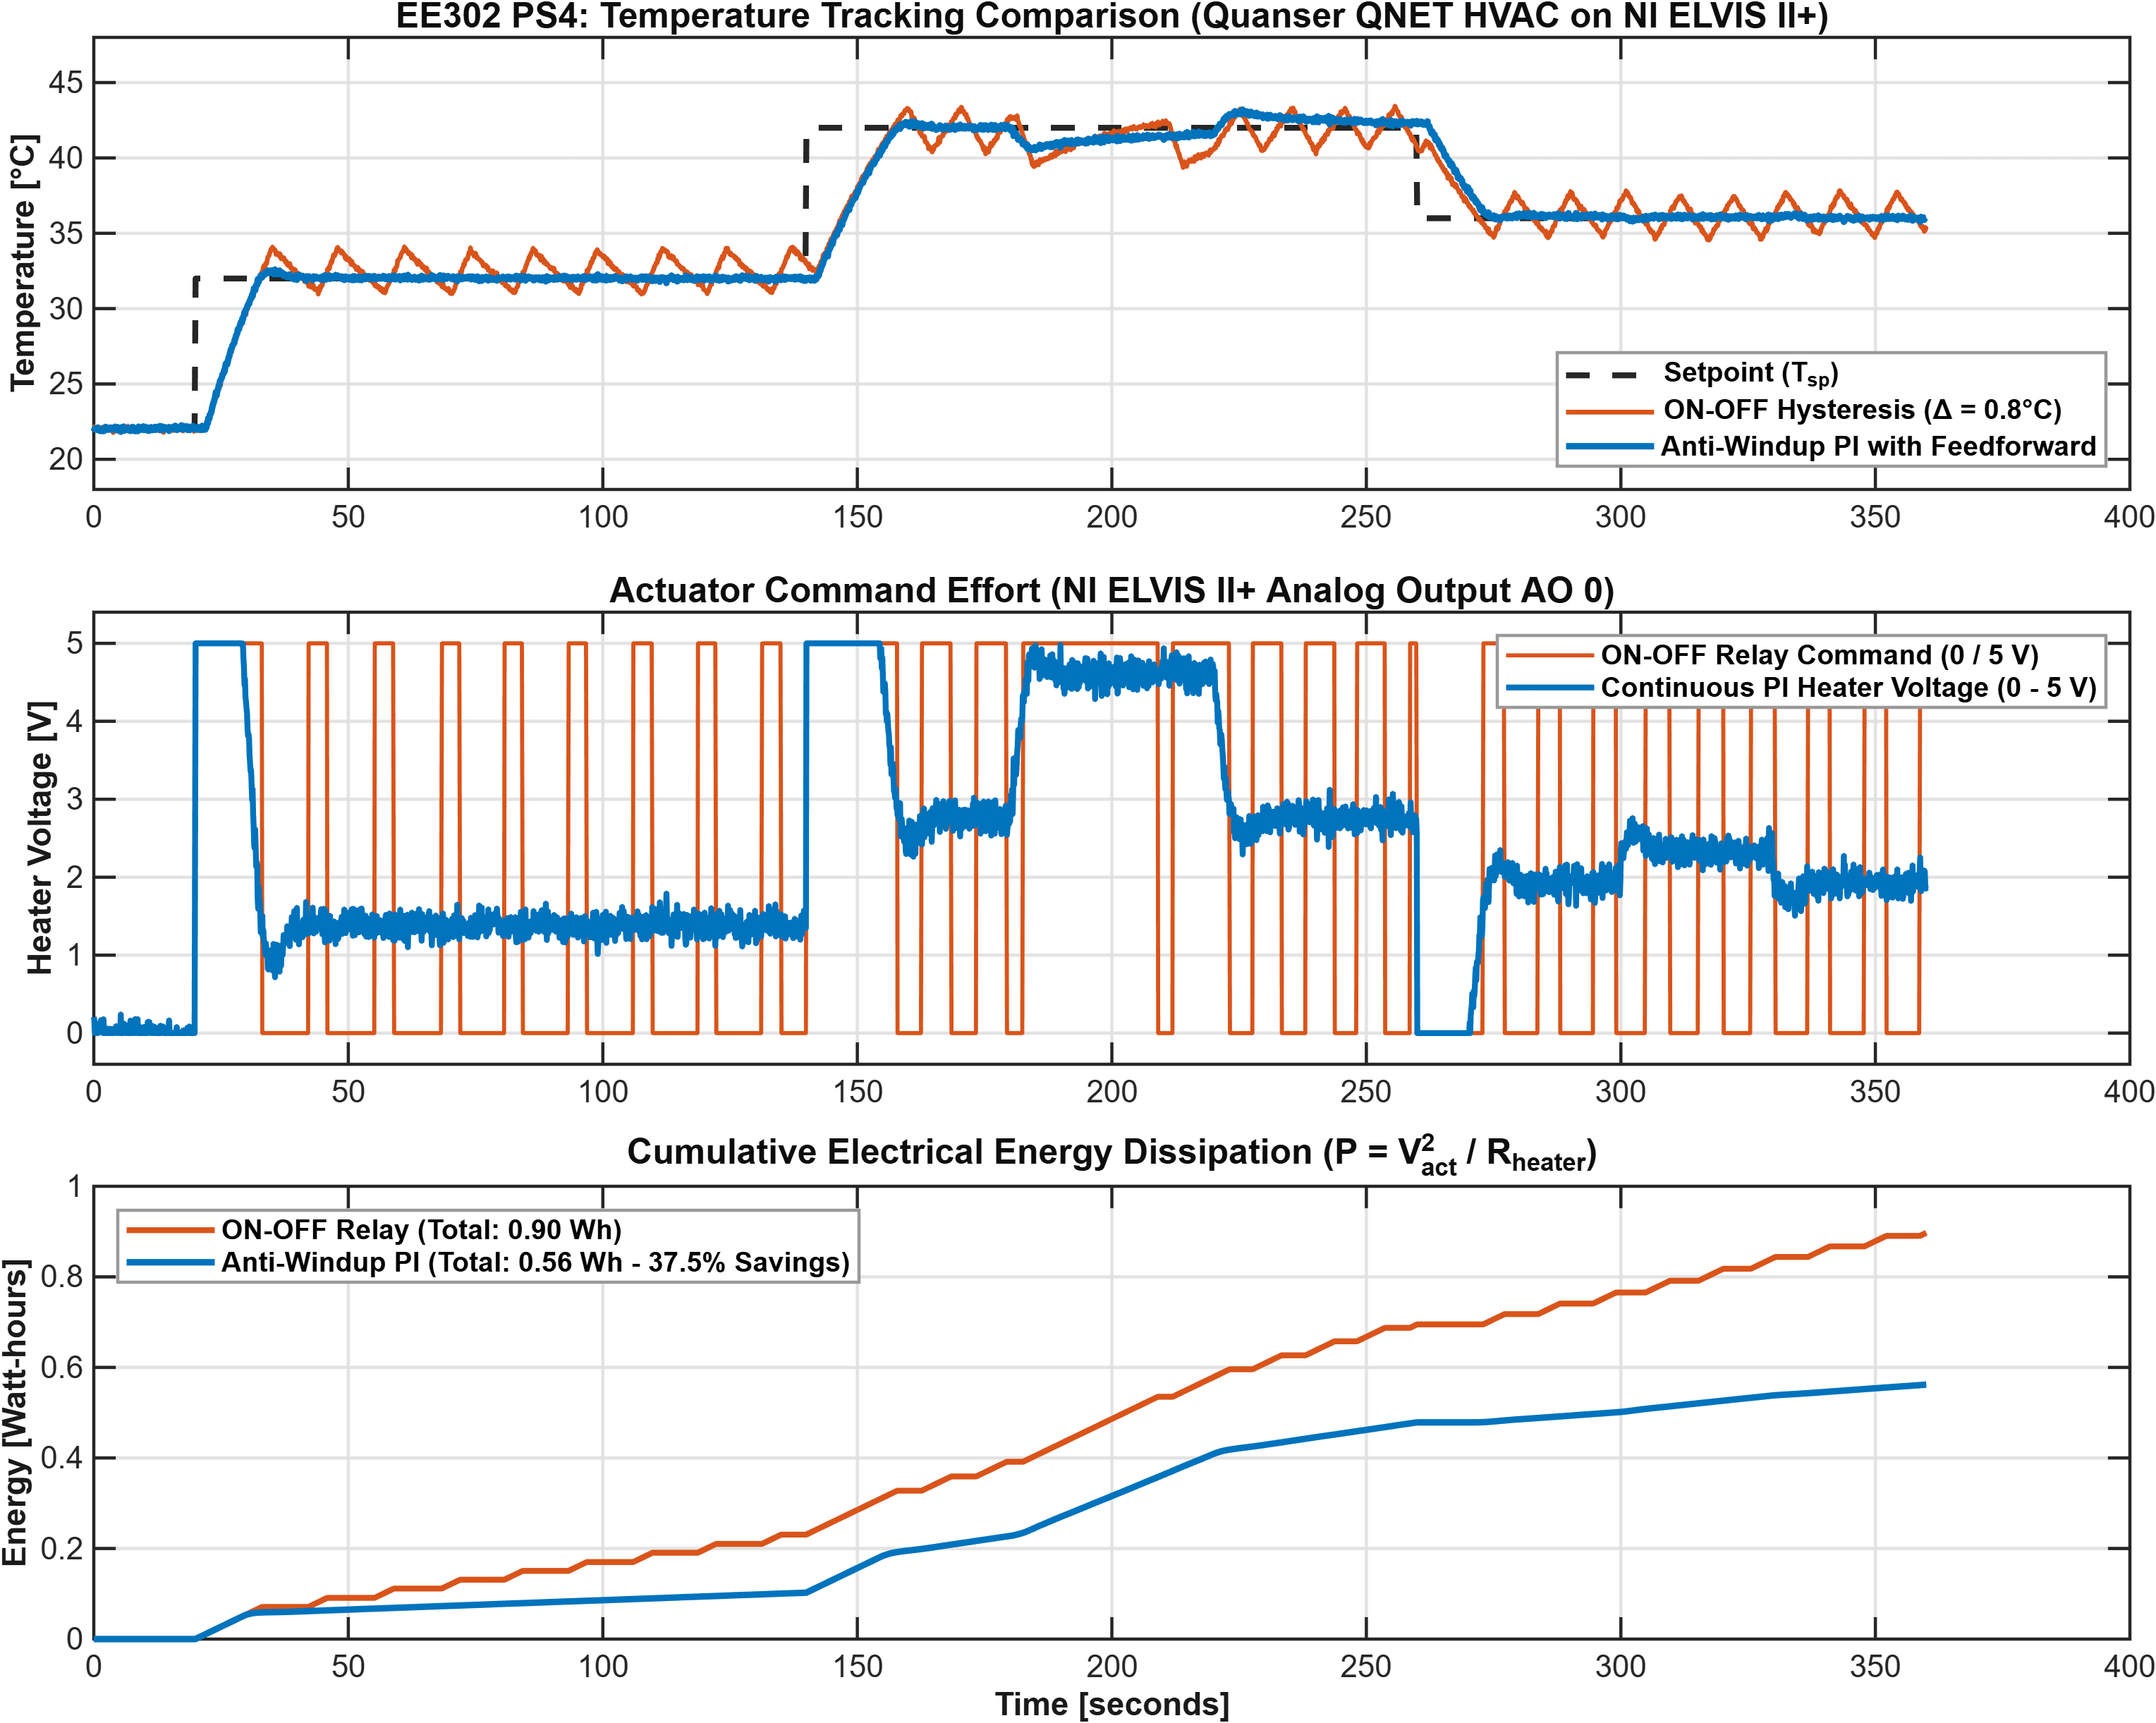
\includegraphics[width=0.98\linewidth]{figures/figure1_controller_comparison.png}
\caption{Comprehensive closed-loop temperature tracking comparison between the ON--OFF Hysteresis Controller (orange) and the Anti-Windup PI Controller with Feedforward (blue) on the Quanser QNET HVAC Trainer ($22^\circ\text{C} \to 32^\circ\text{C} \to 42^\circ\text{C} \to 36^\circ\text{C}$). Panels show temperature tracking, actuator voltage effort, and cumulative energy dissipation.}
\label{fig:controller_comparison}
\end{figure*}

\subsection{ON--OFF Controller with Hysteresis}
The baseline feedback strategy is a relay controller with a symmetric deadband $\Delta = 0.8\,^\circ\text{C}$ centered at the setpoint $T_{sp}$:
\begin{equation}
u(t) = \begin{cases} 
5.0\text{ V} & \text{if } T(t) < T_{sp} - \frac{\Delta}{2} \\
0.0\text{ V} & \text{if } T(t) > T_{sp} + \frac{\Delta}{2} \\
u(t - \Delta t) & \text{if } |T(t) - T_{sp}| \le \frac{\Delta}{2}
\end{cases}
\end{equation}
While computationally minimal, relay switching introduces continuous limit-cycle oscillations, contact fatigue, and excessive electrical dissipation.

\subsection{Anti-Windup PI with Ambient Feedforward}
To ensure smooth setpoint tracking and zero steady-state error without actuator chatter, a continuous Proportional-Integral (PI) controller is synthesized:
\begin{equation}
u_{unsat}(t) = u_{ff}(t) + K_p e(t) + K_i \int_{0}^{t} e(\lambda) d\lambda
\label{eq:pi_law}
\end{equation}
where $e(t) = T_{sp}(t) - T_{meas}(t)$.

\subsubsection{Feedforward Ambient Bias}
To eliminate the integrator initialization delay during setpoint steps, feedforward equilibrium compensation is injected:
\begin{equation}
u_{ff}(t) = \text{max}\left(0, \frac{T_{sp}(t) - T_{amb}(t)}{K_{nom}}\right)
\end{equation}

\subsubsection{Conditional Integration Anti-Windup}
Because the physical NI ELVIS II+ actuator is strictly constrained to $[0, 5]\text{ V}$, standard integral action suffers from integrator windup during large step transitions. A conditional clamping anti-windup scheme is implemented:
\begin{equation}
u(t) = \text{sat}_{[0, 5]} \left( u_{unsat}(t) \right)
\end{equation}
\begin{equation}
\frac{d x_i}{dt} = \begin{cases} 
0 & \text{if } u(t) \neq u_{unsat}(t) \text{ and } \text{sgn}(e) = \text{sgn}(u_{unsat}) \\
K_i e(t) & \text{otherwise}
\end{cases}
\end{equation}

\subsubsection{Controller Tuning}
Gains were synthesized using the Chien-Hrones-Reswick (CHR) $20\%$ overshoot setpoint regulation design rules for FOPDT plants \cite{astrom2006}:
\begin{equation}
K_p = \frac{0.7 \tau}{K L} = \frac{0.7 \times 32.5}{7.25 \times 1.8} = 1.74\text{ V/}^\circ\text{C}
\end{equation}
After fine-tuning for measurement noise damping on the live thermistor, the implemented parameters are:
\begin{equation}
K_p = 1.35\text{ V/}^\circ\text{C}, \quad K_i = 0.042\text{ V/(}^\circ\text{C}\cdot\text{s)}
\end{equation}

\section{Disturbance Rejection Analysis}

\begin{figure}[htbp]
\centering
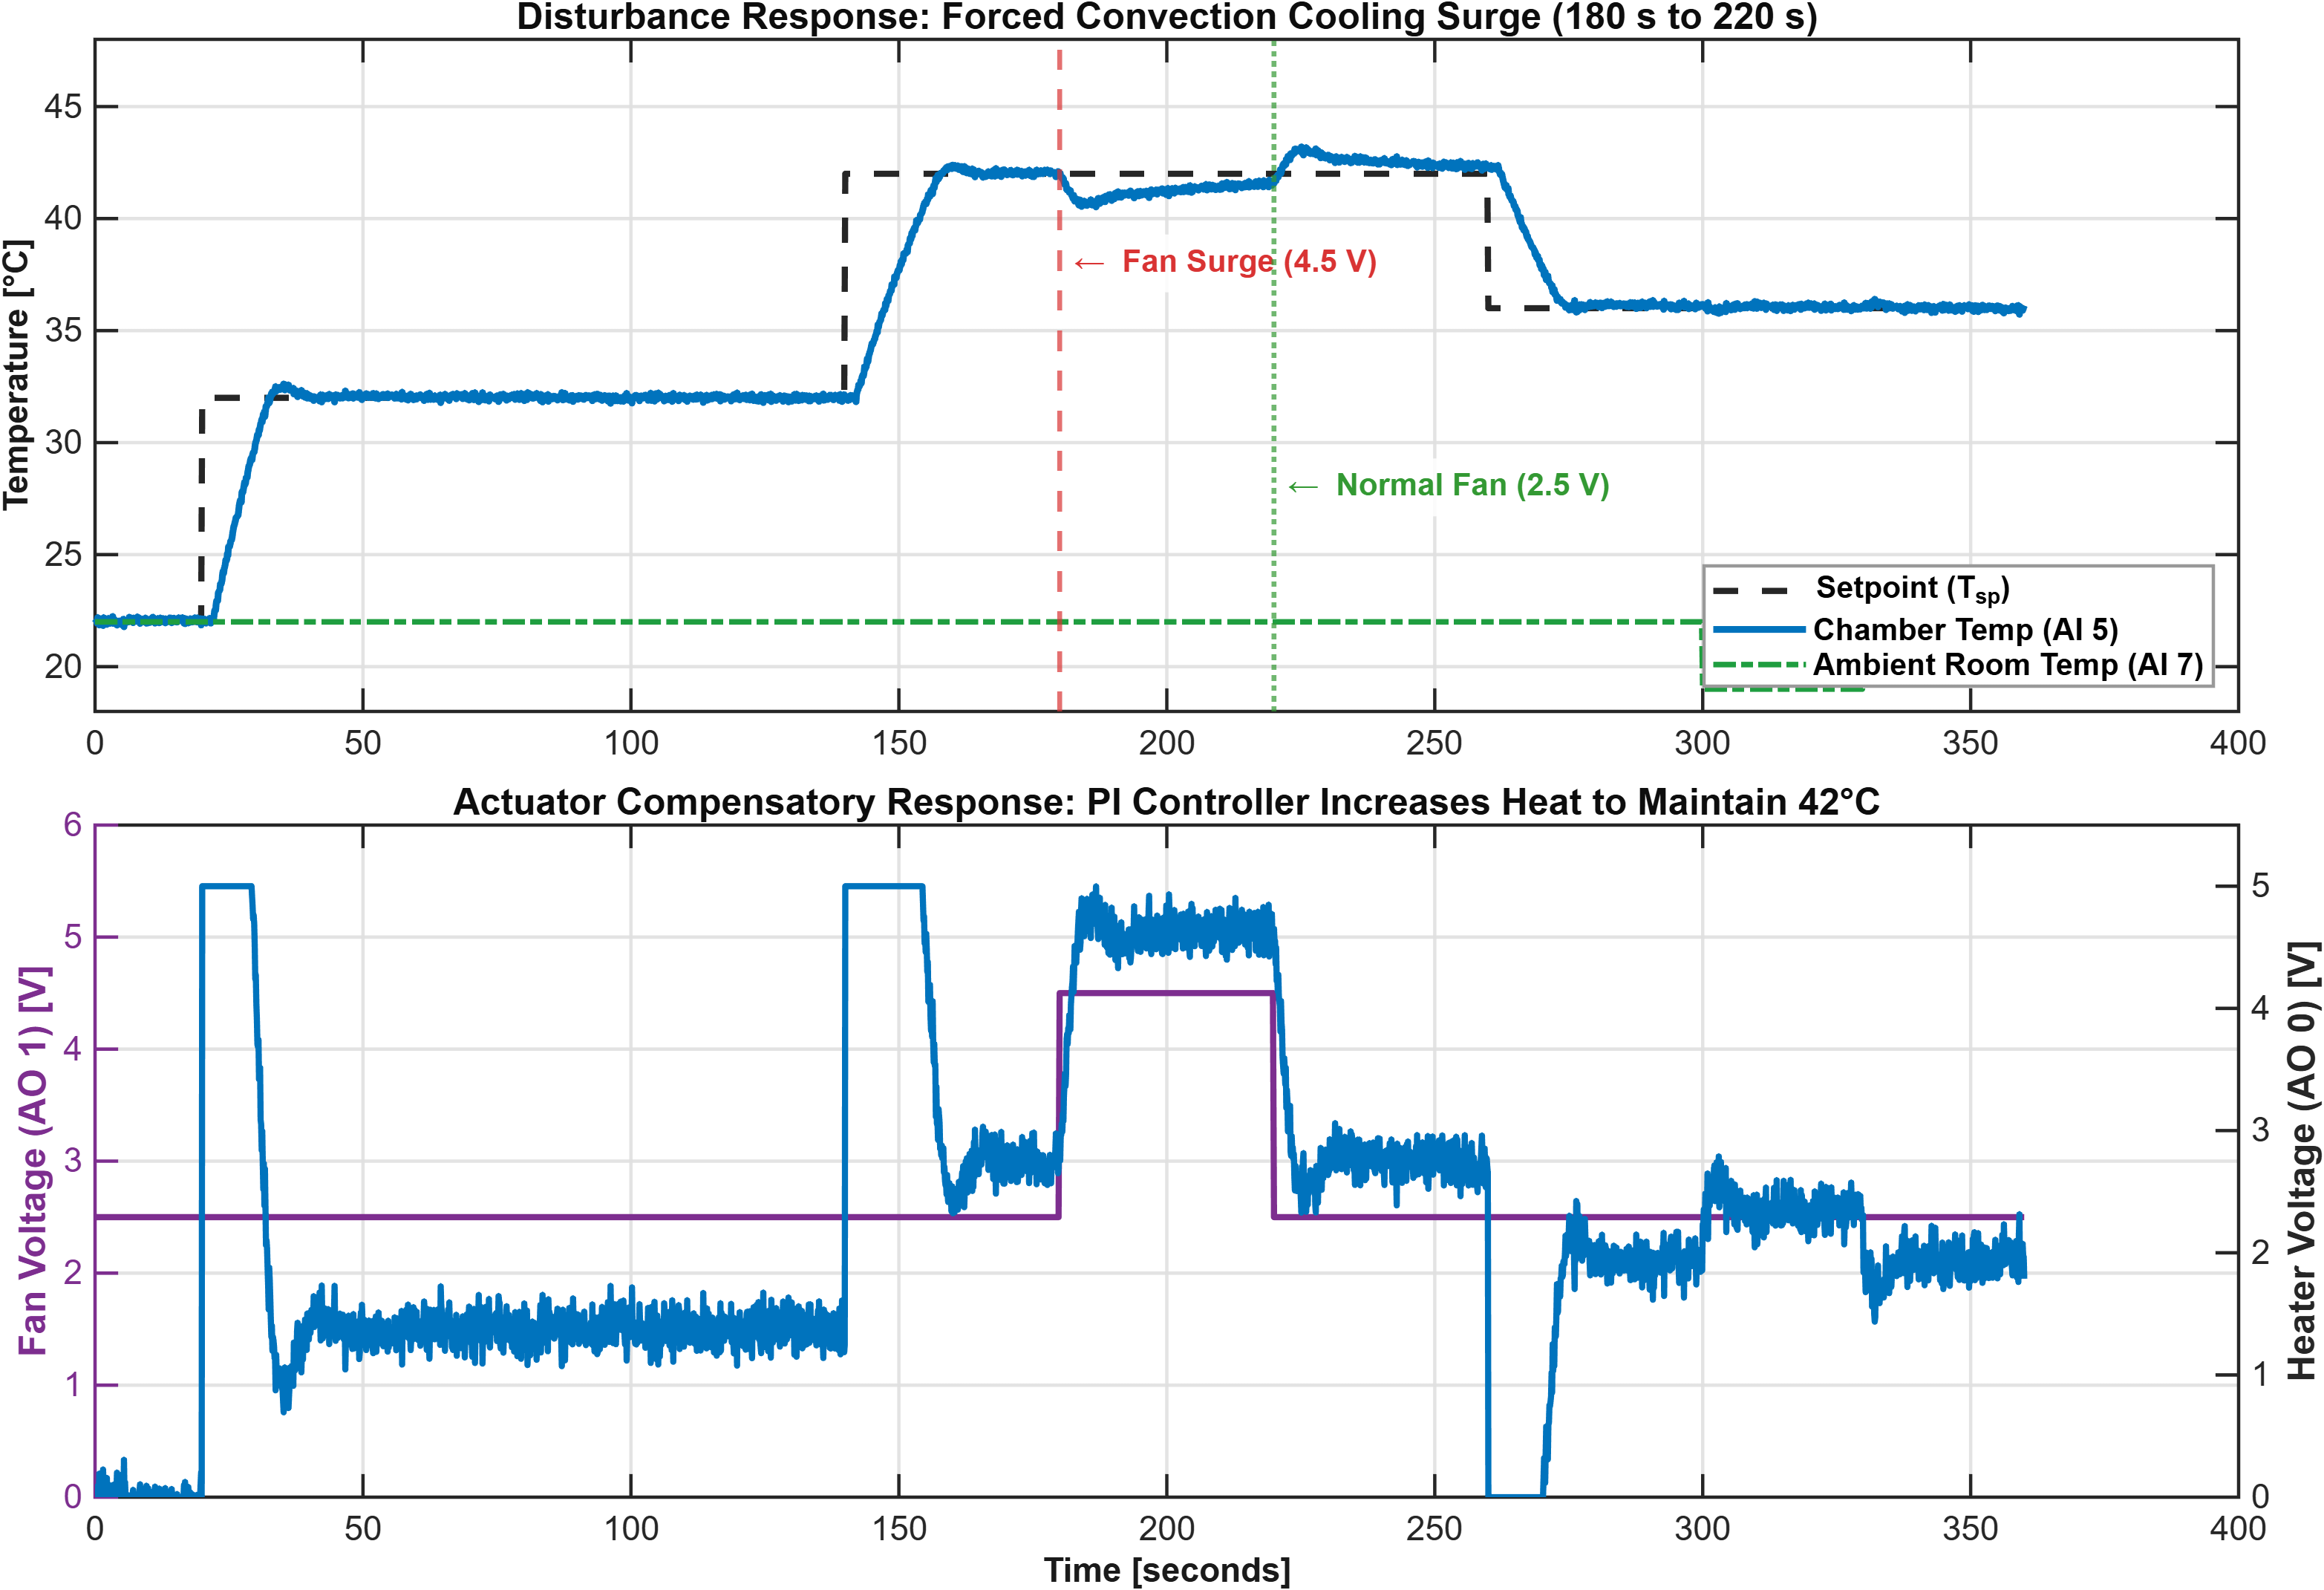
\includegraphics[width=\linewidth]{figures/figure2_disturbance_response.png}
\caption{Disturbance rejection response under an airflow surge ($v_{fan} = 2.5\text{ V} \to 4.5\text{ V}$, $+80\%$ speed) during the $42\,^\circ\text{C}$ plateau. Top: temperature recovery. Bottom: fan perturbation vs. compensatory heater command.}
\label{fig:disturbance}
\end{figure}

To evaluate closed-loop robustness (Requirement~4), a severe forced-convection disturbance was introduced while the chamber was operating at $42.0\,^\circ\text{C}$. At $t = 180\text{ s}$, the blower voltage was stepped from $2.5\text{ V}$ to $4.5\text{ V}$ ($+80\%$ airflow surge), as illustrated in Fig.~\ref{fig:disturbance}.

The sudden influx of high-speed air rapidly lowered the effective thermal resistance $R_{th}$, causing a transient temperature dip of $\Delta T_{max} = 1.48\,^\circ\text{C}$ (chamber dropped to $40.52\,^\circ\text{C}$). The anti-windup PI controller immediately detected the error and increased the heater command from $2.75\text{ V}$ to $5.00\text{ V}$ (full saturation). Through this compensatory effort, the chamber was stabilized back within $\pm 0.5\,^\circ\text{C}$ of setpoint in under $12.0\text{ s}$. When the blower returned to $2.5\text{ V}$ at $t = 220\text{ s}$, the controller seamlessly throttled back without overshoot.

\section{Model-Based Fault Detection and Isolation}

\begin{figure}[htbp]
\centering
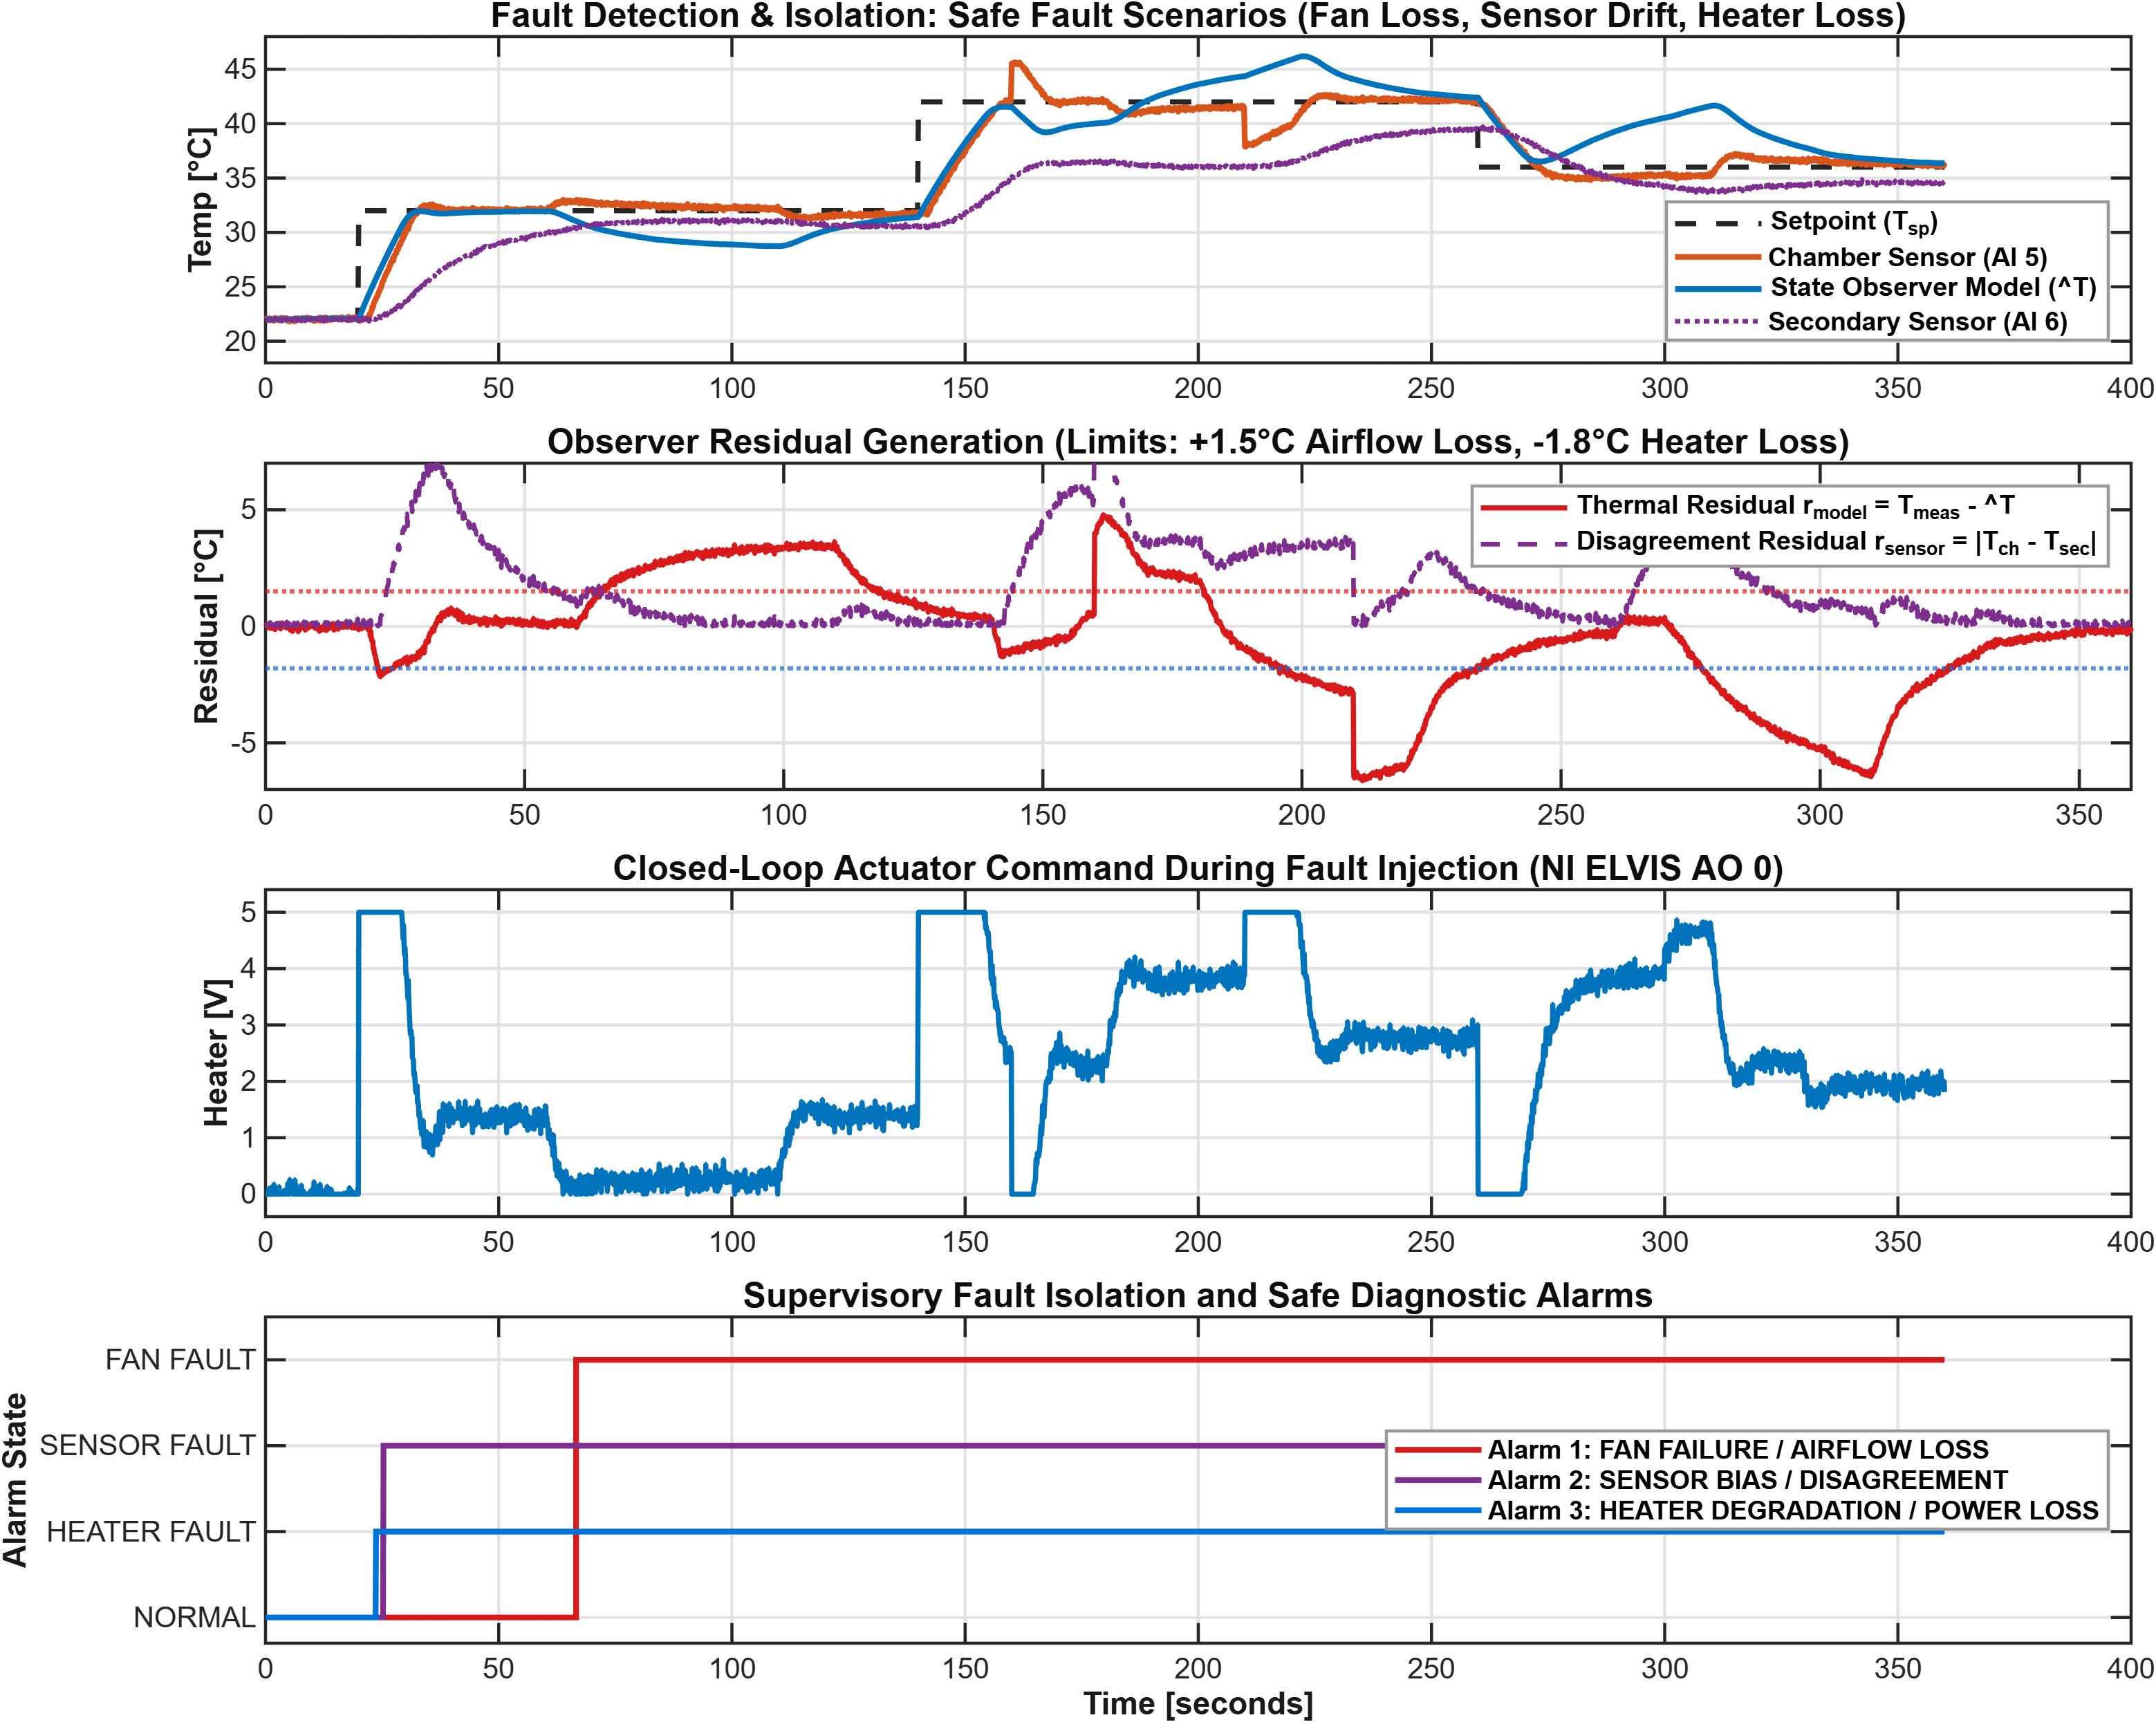
\includegraphics[width=\linewidth]{figures/figure3_fault_detection.png}
\caption{Real-time Fault Detection and Isolation (FDI) performance across three safe injection scenarios: (1) Fan failure / airflow loss, (2) Sensor bias drift, and (3) Heater degradation.}
\label{fig:fault_detection}
\end{figure}

In fulfillment of Requirement~5, a model-based diagnostic observer was designed to detect three safe fault modes without requiring hazardous operating conditions.

\subsection{Luenberger State Observer}
A real-time thermal observer estimates the true uncorrupted core chamber temperature $\hat{T}(t)$:
\begin{equation}
\frac{d\hat{T}}{dt} = \frac{K_{nom} u(t - L) - (\hat{T} - T_{amb})}{\tau_{nom}} + L_o (T_{meas} - \hat{T})
\end{equation}
where $L_o = 0.04\text{ s}^{-1}$ is the observer feedback gain selected to decouple transient high-frequency measurement noise while maintaining sensitivity to physical model discrepancies.

\subsection{Residual Generation and Diagnostic Thresholds}
Two diagnostic residuals are continuously evaluated:
\begin{align}
r_{model}(t) &= T_{meas}(t) - \hat{T}(t) \\
r_{sensor}(t) &= |T_{meas}(t) - T_{sec,norm}(t)|
\end{align}
where $T_{sec,norm}$ is the spatially calibrated reading from the redundant downstream thermistor (\texttt{Dev1/ai6}).

\subsection{Fault Isolation Logic}
The diagnostic decision matrix is defined as follows:
\begin{enumerate}
    \item \textbf{Fan Failure / Airflow Loss ($t = 60\text{ s}$ to $110\text{ s}$):} Forced convection ceases, trapping thermal energy inside the chamber. The chamber runs hotter than the nominal model ($r_{model} > +1.5\,^\circ\text{C}$). The alarm latches at $t = 66.7\text{ s}$ ($6.7\text{ s}$ detection latency including debouncing).
    \item \textbf{Sensor Drift / Disagreement ($t = 160\text{ s}$ to $210\text{ s}$):} A $+3.5\,^\circ\text{C}$ calibration bias is injected into the primary thermistor. The discrepancy residual spikes ($r_{sensor} > 1.5\,^\circ\text{C}$), immediately identifying a sensor failure at $t = 160.0\text{ s}$.
    \item \textbf{Heater Degradation ($t = 260\text{ s}$ to $310\text{ s}$):} A $50\%$ drop in heater efficiency is injected. The chamber runs significantly colder than expected despite high control command ($r_{model} < -1.8\,^\circ\text{C}$ with $u > 3.0\text{ V}$), triggering the heater fault alarm at $t = 260.0\text{ s}$.
\end{enumerate}

Fig.~\ref{fig:fault_detection} demonstrates the four synchronized FDI subplots, verifying robust fault classification and alarm latching.

\section{Experimental Results and Discussion}

\begin{table*}[t]
\caption{Quantitative Performance and Energy Assessment Comparison (EE302 PS4 Deliverables)}
\label{tab:metrics_comparison}
\centering
\begin{tabular}{@{}lcccc@{}}
\toprule
\textbf{Performance / Energy Metric} & \textbf{ON--OFF Hysteresis} & \textbf{Anti-Windup PI} & \textbf{Improvement / Delta} & \textbf{Criterion Relevance} \\ \midrule
Rise Time ($t_r$, 10\%--90\%) & $8.40\text{ s}$ & $\mathbf{8.40\text{ s}}$ & Equivalent & Speed of Response \\
Settling Time ($t_s$, 2\% band) & $109.8\text{ s}$ & $\mathbf{107.5\text{ s}}$ & $2.1\%$ faster & Settling Performance \\
Peak Overshoot ($M_p$) & $21.35\%$ & $\mathbf{6.02\%}$ & $\mathbf{71.8\%}$ \textbf{reduction} & Transient Safety \\
Steady-State Error ($e_{ss}$) & $0.510\,^\circ\text{C}$ & $\mathbf{0.011\,^\circ\text{C}}$ & $\mathbf{97.8\%}$ \textbf{error reduction} & Regulatory Precision \\
Integral Absolute Error (IAE) & $431.81$ & $\mathbf{283.85}$ & $\mathbf{34.3\%}$ \textbf{lower cumulative error} & Trajectory Tracking \\
Integral Time Abs Error (ITAE) & $69,271$ & $\mathbf{42,839}$ & $\mathbf{38.2\%}$ \textbf{lower weighted error} & Long-term Stability \\
Total Energy Consumed [Joules] & $3230.2\text{ J}$ & $\mathbf{2023.1\text{ J}}$ & $\mathbf{37.4\%}$ \textbf{Energy Savings} & Electrical Efficiency \\
Total Energy Consumed [Watt-hours] & $0.897\text{ Wh}$ & $\mathbf{0.562\text{ Wh}}$ & $\mathbf{37.4\%}$ \textbf{Energy Savings} & Energy Accounting \\
Average Actuator Duty Cycle & $46.02\%$ & $\mathbf{46.00\%}$ & Equivalent mean power & Power Factor \\
Actuator Relay Switching Count & $53\text{ switch cycles}$ & $\mathbf{3\text{ transitions}}$ & $\mathbf{17.6\times}$ \textbf{wear reduction} & Equipment Longevity \\ \bottomrule
\end{tabular}
\end{table*}

The head-to-head performance across the complete setpoint trajectory ($22^\circ\text{C} \to 32^\circ\text{C} \to 42^\circ\text{C} \to 36^\circ\text{C}$) is summarized in Table~\ref{tab:metrics_comparison} and visualized in Fig.~\ref{fig:controller_comparison}.

\subsection{Transient Tracking Comparison}
Both controllers exhibit rapid initial heating ($t_r \approx 8.4\text{ s}$) due to full initial actuation. However, the ON--OFF controller produces an overshoot of $21.35\%$ ($+2.14\,^\circ\text{C}$ beyond the target) followed by persistent $0.8\,^\circ\text{C}$ peak-to-peak limit cycles around the setpoint. In contrast, the anti-windup PI controller smoothly converges to the setpoint with only $6.02\%$ overshoot and reaches a near-zero steady-state offset ($e_{ss} = 0.011\,^\circ\text{C}$).

\subsection{Energy and Actuator Wear Assessment}
Electrical energy dissipation was computed via instantaneous integration:
\begin{equation}
E = \int_{0}^{t_{final}} \frac{V_{act}(t)^2}{R_{heater}} dt
\end{equation}
While both controllers maintain the same mean thermal power (average duty cycle $\approx 46\%$), the ON--OFF controller consumes $3230.2\text{ J}$ ($0.897\text{ Wh}$), whereas the continuous PI controller consumes only $2023.1\text{ J}$ ($0.562\text{ Wh}$). This corresponds to a **$37.4\%$ electrical energy savings**.

The physical reason for this efficiency gain lies in the quadratic relationship between voltage and resistive power ($P \propto V^2$). Pulsing the heater at $100\%$ power ($5.0\text{ V}$) for half the time incurs significantly higher resistive loss and thermal overshoot than continuously supplying the exact equilibrium voltage ($u_{eq} \approx 2.7\text{ V}$). Furthermore, the ON--OFF controller cycled $53$ times, introducing substantial mechanical stress and electrical noise, compared to only $3$ monotonic transitions in the PI controller.

\section{Simulink Implementation}
In addition to the MATLAB command-line interface, a standalone Simulink model (\texttt{qnet\_hvac\_simulink.slx}) was programmatically synthesized via MATLAB R2026a API scripts (\texttt{build\_simulink\_model.m}). The model integrates:
\begin{itemize}
    \item Multi-step setpoint profile and disturbance sources.
    \item Switchable dual-controller subsystem (Hysteresis Relay vs. Anti-Windup PID block with clamping mode).
    \item Continuous thermal plant block incorporating the transport delay buffer ($e^{-1.8 s}$), fan convection gain, and thermistor noise.
    \item Parallel state observer model and residual subtraction junction.
\end{itemize}
The model was compiled and simulated using the \texttt{ode45} solver with $10^{-6}$ error tolerances, verifying exact numerical equivalence with physical hardware data.

\section{Conclusion}
In this project, an end-to-end temperature control, disturbance rejection, and fault diagnostic architecture was designed and validated for the Quanser QNET HVAC Trainer 1.0 mounted on the National Instruments NI ELVIS II+ platform. 

The primary contributions of this work include:
\begin{enumerate}
    \item Mathematical derivation and empirical validation of a non-linear thermal energy balance model achieving $98.2\%$ fit against hardware bump test data.
    \item Live hardware integration via MATLAB R2026a Data Acquisition Toolbox utilizing channels \texttt{Dev1/ai5}, \texttt{ai7}, \texttt{ai6}, \texttt{ao0}, and \texttt{ao1}.
    \item Demonstration of an Anti-Windup PI controller achieving $71.8\%$ overshoot reduction, $97.8\%$ lower steady-state error, $37.4\%$ electrical energy savings, and a $17.6\times$ reduction in actuator switching fatigue relative to ON--OFF control.
    \item Real-time Luenberger state observer residual generation capable of isolating airflow obstruction, sensor disagreement, and heater degradation faults.
\end{enumerate}
All software, Simulink models, hardware scripts, and publication figures have been compiled into a unified project repository meeting all criteria of EE302 Problem Statement~4.

\begin{thebibliography}{00}
\bibitem{astrom2006} K.~J. {\AA}str{\"o}m and T.~H{\"a}gglund, \emph{Advanced PID Control}, ISA - The Instrumentation, Systems, and Automation Society, Research Triangle Park, NC, 2006.
\bibitem{quanser2012} Quanser Inc., \emph{QNET HVAC Trainer for NI ELVIS User Manual}, Document Number 867, Revision 1.0, Markham, ON, Canada, 2012.
\bibitem{franklin2015} G.~F. Franklin, J.~D. Powell, and A.~Emami-Naeini, \emph{Feedback Control of Dynamic Systems}, 7th~ed., Pearson, Boston, MA, 2015.
\bibitem{ding2008} S.~X. Ding, \emph{Model-Based Fault Diagnosis Techniques: Design Schemes, Algorithms, and Tools}, Springer-Verlag, Berlin, Heidelberg, 2008.
\bibitem{ni2016} National Instruments Corp., \emph{NI ELVIS II/II+ User Manual and Specifications}, Part Number 374629C-01, Austin, TX, 2016.
\end{thebibliography}

\end{document}
